\part{Plano de Gerenciamento de Riscos}
\chapter[Plano de Gerenciamento de Riscos]{Plano de Gerenciamento de Riscos}

\section{Introdução}

Tomando como base o \cite{pmbok2013guia}, uma atividade muito importante para qualquer plano de trabalho é a elaboração de Plano de Gerenciamento de Riscos. Dentro de qualquer projeto em qualquer área, existem diversos riscos que podem afetar o andamento do mesmo, no caso de projetos na área da tecnologia da informação podem haver tanto riscos negativos quanto positivos e riscos internos e externos, que afetam diretamente todas as características de gerência e desenvolvimento referentes ao sistema. Então, o objetivo geral é de descrever os riscos para assim propor ações que podem minimizá-los ou no caso de positivos, optimiza-los.

\section{Processo de Gerenciamento dos Riscos}

Neste tópico é definido como será realizado o processo de gerência em relação aos requisitos, ou seja, a sequência de atividades que possibilitará o monitoramento dos riscos, a figura \ref{fig:plano} representa o diagrama que demonstra o processo após o planejamento do gerenciamento dos riscos, pois essa atividade que seria a primeira foi realizada na construção geral deste documento.

\begin{figure}[h!]
	\centering
	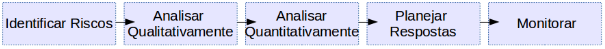
\includegraphics[width=\textwidth]{figuras/plano.png}
	\caption{Processo de gerenciamento dos riscos}
	\label{fig:plano}
\end{figure}

\begin{itemize}
	\item Planejar o Gerenciamento dos Riscos
		\par Nesta fase é definido como as atividades de gerenciamento dos riscos serão dirigidas ao longo do projeto \cite{pmbok2013guia}.
	\item Identificar Riscos
		\par O processo de determinação dos riscos que podem afetar o projeto e de documentação das suas características \cite{pmbok2013guia}.
	\item Analisar Qualitativamente
		\par O processo de priorização de riscos para análise ou ação posterior através da avaliação e combinação de sua probabilidade de ocorrência e impacto \cite{pmbok2013guia}.
	\item Analisar Quantitativamente
		\par O processo de analisar numericamente o efeito dos riscos identificados nos objetivos gerais do projeto.
	\item Planejar Respostas
		\par O processo de desenvolvimento de opções e ações para aumentar as oportunidades e reduzir as ameaças aos objetivos do projeto.
	\item Monitorar
		\par O processo de implementar planos de respostas aos riscos, acompanhar os riscos identificados, monitorar riscos residuais, identificar novos riscos e avaliar a eficácia do processo de gerenciamento dos riscos durante todo o projeto.
\end{itemize}

\section{Metodologia}

A metodologia para o gerenciamento dos riscos será feita de forma informal baseada em reconhecimento de riscos com base na experiência dos integrantes do grupo com projetos passados, na experiência de outros alunos que já participaram de projetos semelhantes ou que já passaram pela disciplina, na própria experiência de trabalho na primeira parte da disciplina e no estudo em cima de projetos parecidos. Será feito uma reunião rápida entre os integrantes do grupo para juntar os dados colhidos e listar os riscos que podem afetar esse projeto.

\section{Papéis e Responsabilidades}

Os papéis e responsabilidades do projeto foram determinadas para que todos os membro do time participem deste processo de gerência, a ideia principal é a de que o grupo, em conjunto direto ou indiretamente, identifique os riscos e que seja feita a análise deles por meio de reuniões. Além dessa identificação, todo o grupo manterá um acompanhamento ou monitoramento de todos os riscos listados ao longo do projeto baseados nas comparações dos resultados de suas ações no projeto com os dados listados nas documentações.

\section{Frequência de Avaliação}

Os riscos apontados neste plano serão revisados em acordo com as datas e períodos definidos no cronograma do projeto. O momento das revisões foram determinados com base nas ideias da metodologia usada que define uma análise ao final de cada fase. Quando for identificado um risco que comprometa o projeto, ele terá uma avaliação imediata pelo grupo de desenvolvimento.

\section{Definições de Probabilidades e impactos de riscos}

Dentro do planejamento do projeto deve-se haver algum tipo de medição para definir o peso dos riscos encontrados em cima do mesmo. A tabela \ref{tab:rel} que possibilitará a criação da matriz de probabilidade, e essa matriz irá disponibilizar dados para quantificação dos riscos. O intervalo definido é em base na probabilidade.

\begin{table}[!h]
\centering
\caption{Relação entre probabilidade, intervalo e peso}
\label{tab:rel}
\resizebox{.5\textwidth}{!}{%
\begin{tabular}{|
>{\columncolor[HTML]{9B9B9B}}c |c|c|}
\hline
Probabilidade & \cellcolor[HTML]{9B9B9B}Intervalo & \cellcolor[HTML]{9B9B9B}Peso \\ \hline
Muito baixa & 1\% -- 20\% & 1 \\ \hline
Baixa & 21\% -- 40\% & 2 \\ \hline
Média & 41\% -- 60\% & 3 \\ \hline
Alta & 61\% -- 80\% & 4 \\ \hline
Muito Alta & 81\% -- 100\% & 5 \\ \hline
\end{tabular}%
}
\end{table}

\section{Matriz de Probabilidade e Impacto}

Na matriz \ref{tab:dist} é definido a distribuição de pesos para as atribuições de impacto e probabilidade

\begin{table}[!h]
\centering
\caption{Distribuição dos pesos entre impacto e probabilidade}
\label{tab:dist}
\resizebox{.8\textwidth}{!}{%
\begin{tabular}{|
>{\columncolor[HTML]{9B9B9B}}c |c|c|c|c|c|}
\hline
Probabilidade/Impacto & \cellcolor[HTML]{9B9B9B}Muito Baixo & \cellcolor[HTML]{9B9B9B}Baixo & \cellcolor[HTML]{9B9B9B}Médio & \cellcolor[HTML]{9B9B9B}Alto & \cellcolor[HTML]{9B9B9B}Muito Alto \\ \hline
Muito baixa & 1 & 2 & 3 & 4 & 5 \\ \hline
Baixa & 2 & 4 & 6 & 8 & 10 \\ \hline
Média & 3 & 6 & 9 & 12 & 15 \\ \hline
Alta & 4 & 8 & 12 & 16 & 20 \\ \hline
Muito Alta & 5 & 10 & 15 & 20 & 25 \\ \hline
\end{tabular}%
}
\end{table}

Tomando como base a matriz \ref{tab:dist} elaborada é possível definir a faixa de peso para as prioridades que pode ser visualizada na tabela \ref{tab:faixa}.

\begin{table}[!h]
\centering
\caption{Faixa de peso para prioridades}
\label{tab:faixa}
\resizebox{.3\textwidth}{!}{%
\begin{tabular}{|
>{\columncolor[HTML]{9B9B9B}}c |c|}
\hline
Prioridade & \cellcolor[HTML]{9B9B9B}Peso \\ \hline
Muito Baixa & 1-5 \\ \hline
Baixa & 6-10 \\ \hline
Média & 11-15 \\ \hline
Alta & 16-20 \\ \hline
Muito Alta & 21-25 \\ \hline
\end{tabular}%
}
\end{table}

\section{Registro dos Riscos}

\subsection{Riscos Negativos}

A tabela \ref{tab:riscneg} apresenta o registro dos riscos negativos do projeto.

\begin{table}[!h]
\centering
\caption{Registo dos riscos negativos do projeto}
\label{tab:riscneg}
\resizebox{\textwidth}{!}{%
\begin{tabular}{|c|c|c|c|}
\hline
\rowcolor[HTML]{9B9B9B} 
Causa & Risco & Descrição & Impacto \\ \hline
Inexperiência com a linguagem & RN01 & Dificuldades na implementação e na arquitetura & Produtividade e entrega do sistema \\ \hline
Inexperiência com as documentações & RN02 & Dificuldades na elaboração dos documentos & Produtividade e entrega dos documentos \\ \hline
Falha na percepção de restrições tecnológicas & RN03 & Não saber o que pode realizar futuramente no projeto & Empacar e atrasar a entrega \\ \hline
Baixo engajamento por parte dos envolvidos no projeto & RN04 & Pouco trabalho realizado por integrantes & Trabalho sobrecarregado \\ \hline
Partes envolvidas não cientes dos desafios do projeto & RN05 & Deixar as atividades para o final do tempo por não saber a complexidade & Não conseguir entregar o sistema \\ \hline
Responsabilidades da equipe de projeto não delineadas & RN06 & Atividades sem responsáveis definidos formalmente & Partes incompletas do trabalho \\ \hline
Cancelamento ou Suspensão do projeto & RN07 & Cancelar o projeto por algum motivo & Não entregar o sistema \\ \hline
Escopo mal planejado & RN08 & Não definir corretamente o escopo & Mudança de escopo e atraso no projeto \\ \hline
Pouca disponibilidade de tempo & RN09 & Integrantes com pouco tempo disponível para trabalhar & Atraso nos tempos do projeto ou atividades sobrecarregadas \\ \hline
Falha no planejamento & RN10 & Planejar o projeto de forma ociosa ou desatenta & Entregas erradas e atraso na entrega \\ \hline
Falha na comunicação com o cliente e na elicitação dos requisitos & RN11 & Produto não atender as expectativas do cliente & Produto não ser utilizado pelo cliente \\ \hline
Desmotivação & RN12 & Baixo rendimento dos integrantes & Atraso nas datas cronograma \\ \hline
Perda dos documentos & RN13 & Perda de todas as informações necessárias para a continuação correta do projeto & Atraso no projeto por haver um novo início ou até seu cancelamento \\ \hline
Perda do código-fonte & RN14 & Perda de todo o código do sistema & Atraso no cronograma e até na entrega \\ \hline
Desistência & RN15 & Integrantes da equipe desistirem da matéria & Atividades sobrecarregadas, mudança de planejamento e atraso no cronograma \\ \hline
\end{tabular}%
}
\end{table}


\subsection{Riscos Positivos}

A tabela \ref{fig:riscposi} apresenta o registro dos riscos positivos do projeto.

\begin{table}[!h]
\centering
\caption{Registo dos riscos positivos do projeto}
\label{fig:riscposi}
\resizebox{\textwidth}{!}{%
\begin{tabular}{|c|c|c|c|}
\hline
\rowcolor[HTML]{9B9B9B} 
Causa & Risco & Descrição & Impacto \\ \hline
Produto bem estruturado & RP01 & O sistema atende perfeitamente todas as necessidades & Cliente desejar continuidade no projeto \\ \hline
Motivação & RP02 & Alto rendimento dos integrantes & Término adiantado de atividades proporcionando revisões \\ \hline
Necessidade de muita documentação & RP03 & A metodologia obriga grande quantidade de documentação & Projeto bem estruturado e organizado \\ \hline
\end{tabular}%
}
\end{table}


\section{Análise e Resposta aos Riscos}
\subsection{Riscos Negativos}

A tabela \ref{fig:respriscneg} apresenta uma resposta de ação com base na análise dos riscos negativos do projeto.

\begin{table}[!h]
\centering
\caption{Análise e resposta aos riscos negativos}
\label{fig:respriscneg}
\resizebox{\textwidth}{!}{%
\begin{tabular}{|c|c|c|c|c|}
\hline
\rowcolor[HTML]{9B9B9B} 
Risco & Probabilidade & Impacto & Prioridade & Ação \\ \hline
RN01 & Muito Alta & Médio & Muito Alta & Mitigar - estudo controlado \\ \hline
RN02 & Muito Alta & Baixo & Muito Alta & Mitigar - estudo controlado \\ \hline
RN03 & Muito Alta & Médio & Muito Alta & Prevenir - estudar tecnologias antes \\ \hline
RN04 & Muito Alta & Alto & Muito Alta & Mitigar - técnicas de motivação \\ \hline
RN05 & Muito Alta & Médio & Muito Alta & Prevenir - estudar projetos parecidos \\ \hline
RN06 & Alta & Alto & Médio & Mitigar - Separar atividades \\ \hline
RN07 & Muito Baixa & Muito Alto & Muito Alta & Independe \\ \hline
RN08 & Alta & Muito Alto & Muito Alta & Prevenir - planejar rigorosamente \\ \hline
RN09 & Média & Alto & Média & Mitigar - definir tempos de trabalho \\ \hline
RN10 & Muito Alta & Muito Alto & Muito Alta & Prevenir - planejar rigorosamente \\ \hline
RN11 & Baixa & Muito Alto & Muito Alta & Prevenir - reuniões bem planejadas \\ \hline
RN12 & Alta & Muito Alto & Média & Mitigar - técnicas de motivação \\ \hline
RN13 & Muito Baixa & Muito Alto & Baixa & Prevenir - fazer no drive e cada um salva em seu computador \\ \hline
RN14 & Muito Baixa & Muito Alto & Baixa & Prevenir - cada um salva em seu computador e github \\ \hline
RN15 & Alta & Muito Alto & Média & Prevenir - procurar sempre ajudar membros com dificuldades \\ \hline
\end{tabular}%
}
\end{table}

\subsection{Riscos Positivos}

A tabela \ref{fig:respriscposi} apresenta uma resposta de ação com base na análise dos riscos positivos do projeto.

\begin{table}[!h]
\centering
\caption{Análise e resposta aos riscos positivos}
\label{fig:respriscposi}
\resizebox{\textwidth}{!}{%
\begin{tabular}{|c|c|c|c|c|}
\hline
\rowcolor[HTML]{9B9B9B} 
Risco & Probabil. & Impacto & Prioridade & Ação \\ \hline
RN01 & Média & Alto & Alta & Maximizar - empenho de todos \\ \hline
RN02 & Média & Alto & Média & Explorar - técnicas de motivação \\ \hline
RN03 & Muito Alta & Muito Alto & Muito Alta & Maximizar - procurar fazer todos os documentos necessários para o projeto \\ \hline
\end{tabular}%
}
\end{table}